\documentclass{beamer}
\usepackage[utf8]{inputenc}
\usepackage[T1]{fontenc}

\setbeamerfont{title}{size=\LARGE}

\title{Git}
\author{Eliška Jégrová}
\date{24.09.2025}

% pro obrázky a kreslení
\usepackage{tikz}
\usetikzlibrary{positioning}
\usepackage{graphicx}
\usepackage{datetime}
\usepackage{svg}

% vlastní příkaz pro tildy
\newcommand{\ts}{\raisebox{-0.25em}{\textasciitilde}}

\begin{document}
	
	\frame{\titlepage}
	
	% 2. slide - Proč Git?
	\begin{frame}{Proč Git?}
		\begin{center}
			
\includegraphics[width=0.9\textwidth]{why_git.png}
		\end{center}
	\end{frame}
	
	% 3. slide - Nový repozitář
	\begin{frame}[fragile]{Nový repozitář}
		
		\begin{itemize}
			\item Repozitář: místo, kde Git uchovává historii projektu
			\item Vytvoření složky a přepnutí do ní:
		\end{itemize}
		
	{\ttfamily\small
		\$ mkdir \ts/repositar \\
		\$ cd \ts/repositar \\
	}
	
		\hspace{0.5cm}
		\begin{itemize}
			\item Inicializace repozitáře
		\end{itemize}
		
	
	{\ttfamily\small
		\$ git init \\
		Initialized empty Git repository in /home/elza/repositar/.git/ \\
	}
		
		\hspace{0.5cm}
		\begin{itemize}
			\item Stav repozitáře
		\end{itemize}
		
	{\ttfamily\small
		\$ git status \\
		On branch main \\
		No commits yet \\
		nothing to commit (create/copy files and use "git add" to track)
	}
		
	\end{frame}
	
	
	
	% 4. slide - Přidání souboru (kontrola stavu)
	\begin{frame}[fragile]{Přidání souboru}
		
		\begin{itemize}
			\item Vytvořte nový soubor  \texttt{basnicka.txt} v \ts/repositar
			\item Nejprve zkontrolujeme stav repozitáře
		\end{itemize}
	
	{\ttfamily\small
		\$ git status \\
		Untracked files: \\
		(use "git add <file>..." to include in what will be committed) \\
		\ \ \textcolor{red}{basnicka.txt}
	}
	
		\begin{center}
		% použití SVG přímo (nutné kompilovat s --shell-escape)
		\includesvg[width=0.7\textwidth]{diagram}
		\end{center}
	
	\end{frame}
	
% 5. slide - Přidání souboru (commit)
\begin{frame}[fragile]{Přidání souboru}
	
	\begin{itemize}
		\item Přidání souboru ke sledování
	\end{itemize}
	
	{\ttfamily\small
		\$ git add basnicka.txt \\
		\$ git status \\
		On branch main
		
		No commits yet
		
		Changes to be committed: \\
		\ \ new file:   \textcolor{green}{basnicka.txt}
	}
	
	\hspace{0.5cm}
	\begin{itemize}
		\item Uložení změn do repozitáře
	\end{itemize}
	
	{\ttfamily\small
		\$ git commit \\
		\texttt{[main (root-commit) 50a3ab8] Přidání básničky} \\
		1 file changed, 2 insertions(+) \\
		create mode 100644 basnicka.txt
	}
	
\end{frame}

	
% 6.a slide - Úprava souboru
\begin{frame}[fragile]{Úprava souboru}
	
	\begin{itemize}
		\item Upravíme obsah souboru \texttt{basnicka.txt}
		\item Zkontrolujeme stav repozitáře
	\end{itemize}
	
	{\ttfamily\small
		\$ git status \\
		On branch main \\
		Changes not staged for commit: \\
		\ \ modified: \textcolor{red}{basnicka.txt} \\
		\ no changes added to commit
	}
	
	\hspace{0.5cm}
	\begin{itemize}
		\item Zobrazíme rozdíly mezi verzemi
	\end{itemize}
	
	{\ttfamily\small
		\$ git diff \\
		diff --git a/basnicka.txt b/basnicka.txt \\
		index 218eee0..306ffa3 100644 \\
		--- a/basnicka.txt \\
		+++ b/basnicka.txt \\
		\textcolor{green}{@@ -1,2 +1,2 @@} \\
		Halo halo, co se stalo? \\
		\textcolor{red}{-Kolo se nám odkutálelo.} \\
		\textcolor{green}{+Kolo se nám polámalo.}
	}
	
\end{frame}


% 6b. slide - Úprava souboru (commit + git show)
\begin{frame}[fragile]{Úprava souboru}
	
	\begin{itemize}
		\item Přidáme změny a uložíme do repozitáře
	\end{itemize}
	
	{\ttfamily\small
		\$ git add basnicka.txt \\
		\$ git commit \\
		\texttt{[main df405e4] Úprava básničky} \\
		1 file changed, 1 insertion(+), 1 deletion(-)
	}
	
	\hspace{0.5cm}
	\begin{itemize}
		\item Zobrazíme podrobnosti o posledním commitu
	\end{itemize}
	
	{\ttfamily\small
		\$ git show \\
\textcolor{orange}{commit} \textcolor{orange}{df405e4ad6615c76e653804f56082d08aa001a2e} (\textcolor{cyan}{HEAD} -> \textcolor{green}{main}) \\

		Author: Eliška Jégrová <eliska@example.com> \\
		Date:   Mon Sep 8 18:14:00 2025 +0200
		
		Úprava básničky

		diff --git a/basnicka.txt b/basnicka.txt \\
		index 218eee0..306ffa3 100644 \\
		--- a/basnicka.txt \\
		+++ b/basnicka.txt \\
		...
	}
	
\end{frame}


% 7. slide - Zobrazení historie
\begin{frame}[fragile]{Jak si zobrazit změny}
	
	\begin{itemize}
		\item Zobrazíme historii commitů
	\end{itemize}
	
	{\ttfamily\small
		\$ git log \\
		
		\textcolor{orange}{commit} \textcolor{orange}{df405e4ad6615c76e653804f56082d08aa001a2e} (\textcolor{cyan}{HEAD} -> \textcolor{green}{main}) \\
		Author: Eliška Jégrová <eliska@example.com> \\
		Date:   Mon Sep 8 18:14:00 2025 +0200
		
		Úprava básničky
		
		\textcolor{orange}{commit} \textcolor{orange}{50a3ab8d9445e3f49bd3353965d5952d73d15124} \\
		Author: Eliška Jégrová <eliska@example.com> \\
		Date:   Mon Sep 8 17:55:38 2025 +0200
		
		První revize
	}
	
	
	\hspace{0.5cm}
	\begin{itemize}
		\item Historii lze zobrazit i graficky či v terminálu:
		\begin{itemize}
			\item \texttt{gitk} – grafické zobrazení commitů
			\item \texttt{tig} – textové terminálové rozhraní
		\end{itemize}
	\end{itemize}
	
\end{frame}


% 8a. slide - Větvení v Gitu (seznam větví)
\begin{frame}[fragile]{Větvení v Gitu}
	\vspace{-1.3cm} % posune obrázek nahoru
	\begin{center}
		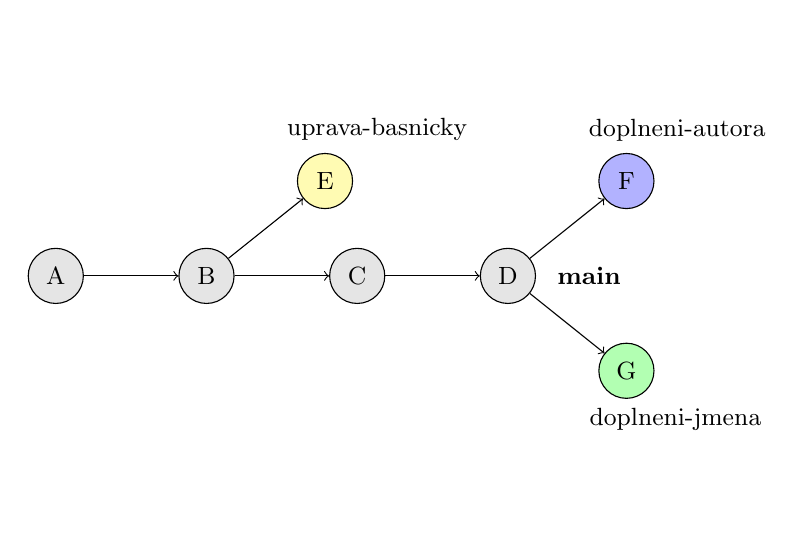
\begin{tikzpicture}[node distance=1.2cm, every node/.style={circle,draw,minimum size=0.7cm, font=\small}]
			% hlavní větev
			\node[fill=black!10] (A) {A};
			\node[fill=black!10,right=of A] (B) {B};
			\node[fill=black!10,right=of B] (C) {C};
			\node[fill=black!10,right=of C] (D) {D};
			
			% větev uprava-basnicky z B
			\node[fill=yellow!30,above right=0.7cm and 1cm of B] (E) {E};
			
			% větev doplneni-autora z D
			\node[fill=blue!30,above right=0.7cm and 1cm of D] (F) {F};
			
			% větev doplneni-jmena z D
			\node[fill=green!30,below right=0.7cm and 1cm of D] (G) {G};
			
			% šipky hlavní větve
			\draw[->] (A)--(B);
			\draw[->] (B)--(C);
			\draw[->] (C)--(D);
			
			% šipky vedlejších větví
			\draw[->] (B)--(E);
			\draw[->] (D)--(F);
			\draw[->] (D)--(G);
			
			% popisky větví
			\node[above right=0.7cm and 1cm of D, draw=none, fill=none] {doplneni-autora};
			\node[below right=0.7cm and 1cm of D, draw=none, fill=none] {doplneni-jmena};
			\node[above right=0.7cm and 1cm of B, draw=none, fill=none] {uprava-basnicky};
			\node[right=0.1cm of D, draw=none, fill=none] {\textbf{main}};
		\end{tikzpicture}
	\end{center}
	
	\vspace{-1.0cm}
	
	\begin{itemize}
		\item Zobrazíme seznam větví
	\end{itemize}
	
	{\ttfamily\small
		\$ git branch \\
		\textcolor{green}{* main}

	}
\end{frame}

% 8b. slide - Větvení v Gitu (práce s větvemi)
\begin{frame}[fragile]{Větvení v Gitu}
	
	\begin{itemize}
		\item Vytvoříme a přepneme se do nové větve pro doplnění autora
	\end{itemize}
	
	{\ttfamily\small
		\$ git branch doplneni-autora \\
		\$ git switch doplneni-autora
	}
	
	\hspace{0.5cm}
	\begin{itemize}
		\item Přepneme zpět na main a vytvoříme větev pro doplnění jména
	\end{itemize}
	
	{\ttfamily\small
		\$ git switch main \\
		\$ git branch doplneni-jmena \\
		\$ git switch doplneni-jmena
	}
	
	\hspace{0.5cm}
	\begin{itemize}
		\item Kontrola větví a commitů
	\end{itemize}
	
	{\ttfamily\small
		\$ gitk {-}{-}all
	}
	
\end{frame}
	

% 9a. slide - Sloučení větví (diagram s merge commit)
\begin{frame}[fragile]{Sloučení větví pomocí git merge}
		\vspace{-1.3cm} % posune obrázek nahoru
	\begin{center}
		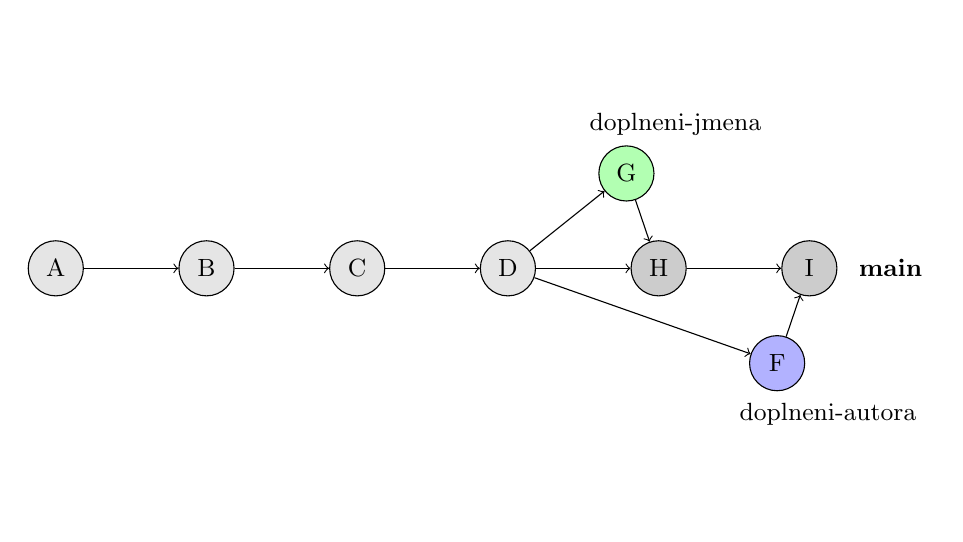
\begin{tikzpicture}[node distance=1.2cm, every node/.style={circle,draw,minimum size=0.7cm, font=\small}]
			
			% hlavní větev
			\node[fill=black!10] (A) {A};
			\node[fill=black!10,right=of A] (B) {B};
			\node[fill=black!10,right=of B] (C) {C};
			\node[fill=black!10,right=of C] (D) {D};
			
			% větev doplneni-jmena z D
			\node[fill=green!30,above right=0.7cm and 1cm of D] (G) {G};
			
			% merge commit po sloučení doplneni-jmena
			\node[fill=black!20,right=of D] (H) {H};
			
			% větev doplneni-autora z D
			\node[fill=blue!30,below right=0.7cm and 1cm of H] (F) {F};
			
			% merge commit po sloučení doplneni-autora
			\node[fill=black!20,right=of H] (I) {I};
			
			% šipky hlavní větve
			\draw[->] (A)--(B);
			\draw[->] (B)--(C);
			\draw[->] (C)--(D);
			
			% šipky vedlejších větví
			\draw[->] (D)--(G);
			\draw[->] (D)--(F);
			
			% merge šipky
			\draw[->] (D)--(H);
			\draw[->] (G)--(H);
			\draw[->] (H)--(I);
			\draw[->] (F)--(I);
			
			% popisky větví
			\node[above right=0.7cm and 1cm of D, draw=none, fill=none] {doplneni-jmena};
			\node[below right=0.7cm and 1cm of H, draw=none, fill=none] {doplneni-autora};
			\node[right=0.1cm of I, draw=none, fill=none] {\textbf{main}};
			
		\end{tikzpicture}
	\end{center}
			\vspace{-1.3cm} % posune obrázek nahoru
		\begin{itemize}
		\item Přepneme se na hlavní větev \textbf{main}, do které chceme sloučit změny
	\end{itemize}
	
	{\ttfamily\small
		\$ git switch main
	}
	
\end{frame}
	
	
% 9. slide - Sloučení větví
\begin{frame}[fragile]{Sloučení větví pomocí git merge}
	

	\hspace{0.5cm}
	\begin{itemize}
		\item Sloučíme změny z vedlejších větví
	\end{itemize}
	
	{\ttfamily\small
		\$ git merge doplneni-jmena \\
		\$ git merge doplneni-autora
	}
	
	\hspace{0.5cm}
	\begin{itemize}
		\item Řešení případného konfliktu (pokud nějaký nastane)
	\end{itemize}
	
	{\ttfamily\small
		\$ git status \\
		\$ git diff \\
		\# Uděláme správné úpravy \\
		\$ git add basnicka.txt \\
		\$ git commit
	}
	
	\hspace{0.5cm}
	\begin{itemize}
		\item Kontrola historie a odstranění dočasných větví
	\end{itemize}
	
	{\ttfamily\small
		\$ gitk --all \\
		\$ git branch {-}{-}delete doplneni-autora \\
		\$ git branch {-}{-}delete doplneni-jmena
	}
	
\end{frame}


% Obrázek - práce se vzdáleným repozitářem s branch a PR
\begin{frame}[fragile]{Práce se vzdáleným repozitářem}
	\begin{center}
		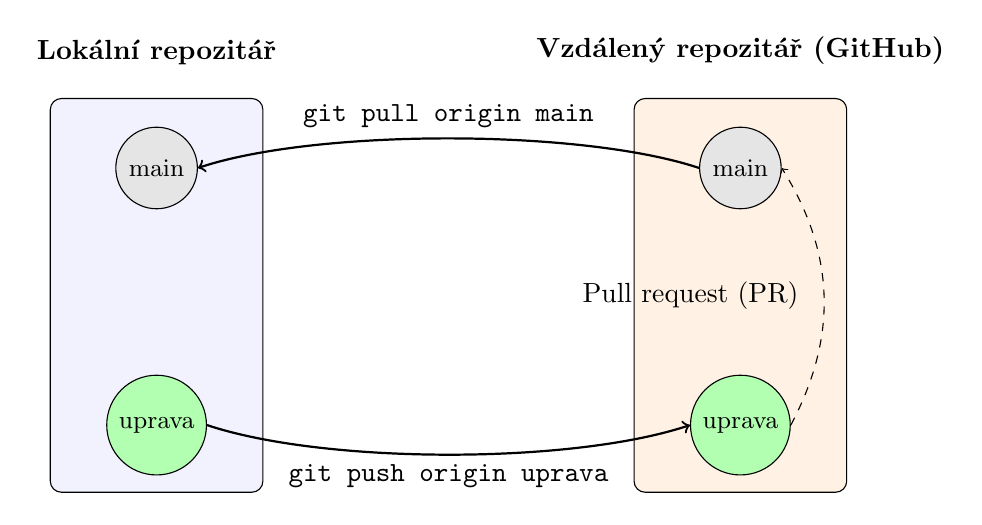
\begin{tikzpicture}[
			repo/.style={rectangle, draw, rounded corners, minimum width=2.7cm, minimum height=5cm, align=center},
			branch/.style={circle, draw, minimum size=0.7cm, font=\small},
			arrow/.style={->, thick}
			]
			
			% Lokální repozitář obdélník + popisek nad ním
			\node[repo, fill=blue!5] (local) {};
			\node[above=0.3cm of local] {\textbf{Lokální repozitář}};
			
			% Větve v lokálním repozitáři (posunuto o 1 cm nahoru)
			\node[branch, fill=black!10, above=3.6cm of local.south] (lmain) {main};
			\node[branch, fill=green!30, below=2.1cm of lmain] (lfeat) {uprava};
			
			% Vzdálený repozitář obdélník + popisek nad ním
			\node[repo, fill=orange!10, right=4.7cm of local] (remote) {};
			\node[above=0.3cm of remote] {\textbf{Vzdálený repozitář (GitHub)}};
			
			% Větve ve vzdáleném repozitáři (posunuto o 1 cm nahoru)
			\node[branch, fill=black!10, above=3.6cm of remote.south] (rmain) {main};
			\node[branch, fill=green!30, below=2.1cm of rmain] (ruprava) {uprava};
			
			% Šipky push/pull - obrácené oblouky
			\draw[arrow] (lfeat.east) .. controls +(1.5,-0.5) and +(-1.5,-0.5) .. node[below, sloped]{\texttt{git push origin uprava}} (ruprava.west);
			\draw[arrow] (rmain.west) .. controls +(-1.5,0.5) and +(1.5,0.5) .. node[above, sloped]{\texttt{git pull origin main}} (lmain.east);
			
			% Pull request ve vzdáleném repozitáři, popisek doprostřed šipky
			\draw[->, dashed, bend right=30] 
			(ruprava.east) 
			to 
			node[midway, left,xshift=-2mm]{Pull request (PR)} 
			(rmain.east);
			

		\end{tikzpicture}
	\end{center}
\end{frame}



	
% 10a. slide - Vzdálený repozitář (klonování)
\begin{frame}[fragile]{Vzdálený repozitář}
	
	\begin{itemize}
		\item Přesun do domovského adresáře
	\end{itemize}
	
	{\ttfamily\small
		\$ cd \ts \\
	}
	
	\hspace{0.5cm}
	\begin{itemize}
		\item Klonování vzdáleného repozitáře z GitHubu
	\end{itemize}
	
	{\ttfamily\small
		\$ git clone git@github.com:PyLadiesCZ-Brno/2025-podzim-linuxadmin-git.git \\
		Cloning into '2025-podzim-linuxadmin-git'... \\
		remote: Enumerating objects: 10, done. \\
		remote: Counting objects: 100\% (10/10), done. \\
		remote: Compressing objects: 100\% (8/8), done. \\
		remote: Total 10 (delta 2), reused 0 (delta 0), pack-reused 0 \\
		Receiving objects: 100\% (10/10), done. \\
	}
	
	\hspace{0.5cm}
	\begin{itemize}
		\item Přepnutí do nově naklonovaného repozitáře
	\end{itemize}
	
	{\ttfamily\small
		\$ cd 2025-podzim-linuxadmin-git \\
	}
	
\end{frame}

% 10b. slide - Vzdálený repozitář (práce se změnami)
\begin{frame}[fragile]{Vzdálený repozitář}
	
	\begin{itemize}
		\item Zobrazení nastaveného vzdáleného repozitáře
	\end{itemize}
	
	{\ttfamily\small
		\$ git remote -v \\
		origin  git@github.com:PyLadiesCZ-Brno/2025-podzim-linuxadmin-git.git (fetch) \\
		origin  git@github.com:PyLadiesCZ-Brno/2025-podzim-linuxadmin-git.git (push) \\
	}
	
	\hspace{0.5cm}
	\begin{itemize}
		\item Odeslání lokálních změn na GitHub
	\end{itemize}
	
	{\ttfamily\small
		\$ git push origin tvoje-vetev \\

	}
	
	\hspace{0.5cm}
	\begin{itemize}
		\item Stažení aktuálních změn z GitHubu
	\end{itemize}
	
	{\ttfamily\small
		\$ git pull origin main \\

	}
\end{frame}

	
\end{document}
